\documentclass[9pt,twocolumn,twoside]{Gunadarma}
\setboolean{shortarticle}{false}


\title{\begin{center}
		Penggunaan Aplikasi \textit{Selenium} Untuk \textit{Automatic Testing} Pada Metodologi \textit{DevOps}
	\end{center}}

\author[1]{Candra Gunawan}
\affil[1]{Magister Manajement Sistem Informasi, Universitas Gunadarma, 2016, Jakarta}
\affil[1]{Corresponding author: sherard@outlook.com}

\author[2]{Deny Pratama}
\affil[2]{Magister Manajement Sistem Informasi, Universitas Gunadarma, 2016, Jakarta}
\affil[2]{Corresponding author: denyuno@gmail.com}

\author[3]{Dewi Apriyani}
\affil[3]{Magister Manajement Sistem Informasi, Universitas Gunadarma, 2016, Jakarta}
\affil[3]{Corresponding author: uwiart93@gmail.com}

\author[4]{Putri Sari Sigiro}
\affil[4]{Magister Manajement Sistem Informasi, Universitas Gunadarma, 2016, Jakarta}
\affil[4]{Corresponding author: putri.sigiro@gmail.com}

\author[5]{Anesia Puji Kinanti}
\affil[5]{Magister Manajement Sistem Informasi, Universitas Gunadarma, 2016, Jakarta}
\affil[5]{Corresponding author: Anesiaakinanti@gmail.com}

\dates{Compiled using \LaTeX\ \today}


\ociscodes{}

\doi{\url{http://Gunadarma.ac.id}}

\begin{abstract}
\textit{DevOps} adalah suatu metode pengembangan \textit{software} yang menekankan komunikasi, kolaborasi dan integrasi antara pengembang \textit{software} dan profesional TI dengan menjadikan proses pembuatan \textit{software} dan perubahan infrastruktur secara otomatis. Metode ini merupakan implementasi dari \textit{"Agile Infrastructure"} yang sebelum nya sudah diperkenalkan. \textit{Selenium} IDE adalah \textit{Integrated Tool} untuk agile testing. Mekanismenya bekerja dengan mereka semua aktifitas user saat mengakses suatu aplikasi berbasis web. Dan selanjut nya, test bisa dilakukan secara otomatis. Tool ini merupakan salah satu tool pendukung di dalam \textit{DevOps}, yaitu untuk melakukan \textit{Test Automation}.  


\end{abstract}

\setboolean{displaycopyright}{true}

\begin{document}

\maketitle
\thispagestyle{fancy}
\ifthenelse{\boolean{shortarticle}}{\abscontent}{}

\section{Pendahuluan}
\subsection{Latar Belakang Masalah}


\textit{Agile} merupakan salah satu metodologi yang diperkenalkan untuk menutup kekurangan metodologi tradisional. Dimana prinsip dari Agile adalah mampu ber-adaptasi terhadap perubahan kebutuhan / (\textit{Requirement}). \textit{Agile} sebagai metodologi, dapa di implementasikan di berbagai macam kebutuhan. Untuk menunjang metodologi \textit{Agile} ini, maka diperlukan berbagai macam tool yang bisa digunakan oleh praktisi \textit{Agile}. Untuk menunjang metode \textit{Agile} tersebut, maka diperlukan suatu alat penunjang. Maka, para praktisi \textit{Agile} sepakat untuk membuat yang disebut \textit{Agile Infrastructure}. 

\textit{Agile Infrastructure} adalah suatu cara mendefinisikan berbagai macam alat / \textit{tools} baik berupa software, hardware maupun proses yang dapat menunjang \textit{Agile}. Dengan \textit{Agile Infrastructure}, diharapkan bisa menunjang agar proses \textit{Agile} bisa lebih efisien. Pertama kali, \textit{Agile Infrastructure} ini diperkenalkan oleh Patrick Debois pada 2009. Dan akhirnya, saat ini lebih dikenal dengan \textit{DevOps}. 

\textit{Devops} adalah metode pengembangan \textit{software} yang menekankan komunikasi, kolaborasi dan integrasi antara pengembang \textit{softwware} dan profesional TI dengan menjadikan proses pembuatan \textit{software} dan perubahan infrastruktur secara otomatis. Adopsi dari \textit{DevOps} ini mencakup :

\begin{itemize}
	\item Menggunakan \textit{Agile} sebagai metodologi
	\item Terdapat nya kebutuhan untuk mempercepat waktu pengembangan aplikasi
	\item \textit{Wide Availability} dan penggunaan \textit{cloud}  infrastructure
	\item Proses otomatis \textit{Environment} dan konfigurasi
	\item Proses testing otomatis dan \textit{Continuous Integration}
\end{itemize}
Dari area \textit{DevOps} di atas, dalam penulisan ini yang dibahas adalah proses testing otomatis / \textit{Automation Testing}. Tool yang akan digunakan adalah \textit{Selenium Web Browser}. 

\textit{Selenium Web Browser} adalah salah satu contoh \textit{tool} untuk melakukan \textit{automated test} untuk aplikasi web. Jadi dengan tool ini, aplikasi web dapat dilakukan test secara otomatis. 



\subsection{Rumusan Masalah}
Rumusan masalah pada jurnal \textbf{"Penggunaan Aplikasi \textit{Selenium} Untuk \textit{Automatic Testing} Pada Metodologi \textit{DevOps}"} adalah untuk menjelasakan bagaimana implementasi \textit{automated testing} dengan menggunakan \textit{tool selenium}  dan kaitan nya dengan metodologi \textit{DevOps}. 


\subsection{Tujuan Penulisan}
Tujuan penulisan ini adalah untuk menjelaskan implementasi dari \textit{DevOps }di salah satu area, yaitu area \textit{testing}. Dimana untuk tool yang digunakan adalah selenium. 


\section{Landasan Teori}

\subsection{Capability Maturity Model}
\textit{Capabilty Maturity Model} disingkat \textbf{CMM} adalah suatu model kematangan kemampuan (kapabilitas) proses yang dapat membantu pendefinisian dan pemahaman proses - proses suatu organisasi. Pengembangan model ini dimulai pada tahun 1986 oleh \textbf{SEI} \textit{(Software Enginering Institute)}. CMM awalnya digunakan sebagai alat ukur untuk secara objectif menilai kemampuan dalam menangani proyek perangkat lunak, dan diharapkan dapat digunakan sebagai suatu model umum untuk membantu pemahaman kematangan kapabilitas proses organisasi. 

\begin{figure}[htbp]
	\begin{center}
		\includegraphics[width=1\columnwidth]{CMM.eps} \label{fig:1-noFCase1}
	\end{center}
	\caption{Capability Maturity Model}
\end{figure}


\subsection{Agile Development Method}
\textbf{\textit{Agile Development Methods}} adalah sekelompok metodologi pengembangan perangkat lunak yang didasarkan pada prinsip-prinsip yang sama atau pengembangan sistem jangka pendek yang memerlukan adaptasi cepat dari pengembang terhadap perubahan dalam bentuk apapun. Agile development methods merupakan salah satu dari Metodologi pengembangan perangkat lunak yang digunakan dalam pengembangan perangkat lunak. Agile memiliki pengertian bersifat cepat, ringan, bebas bergerak, dan waspada. Sehingga saat membuat perangkat lunak dengan menggunakan agile development methods diperlukan inovasi dan responsibiliti yang baik antara tim pengembang dan klien agar kualitas dari perangkat lunak yang dihasilkan bagus dan kelincahan dari tim seimbang.

\begin{figure}[htbp]
\begin{center}
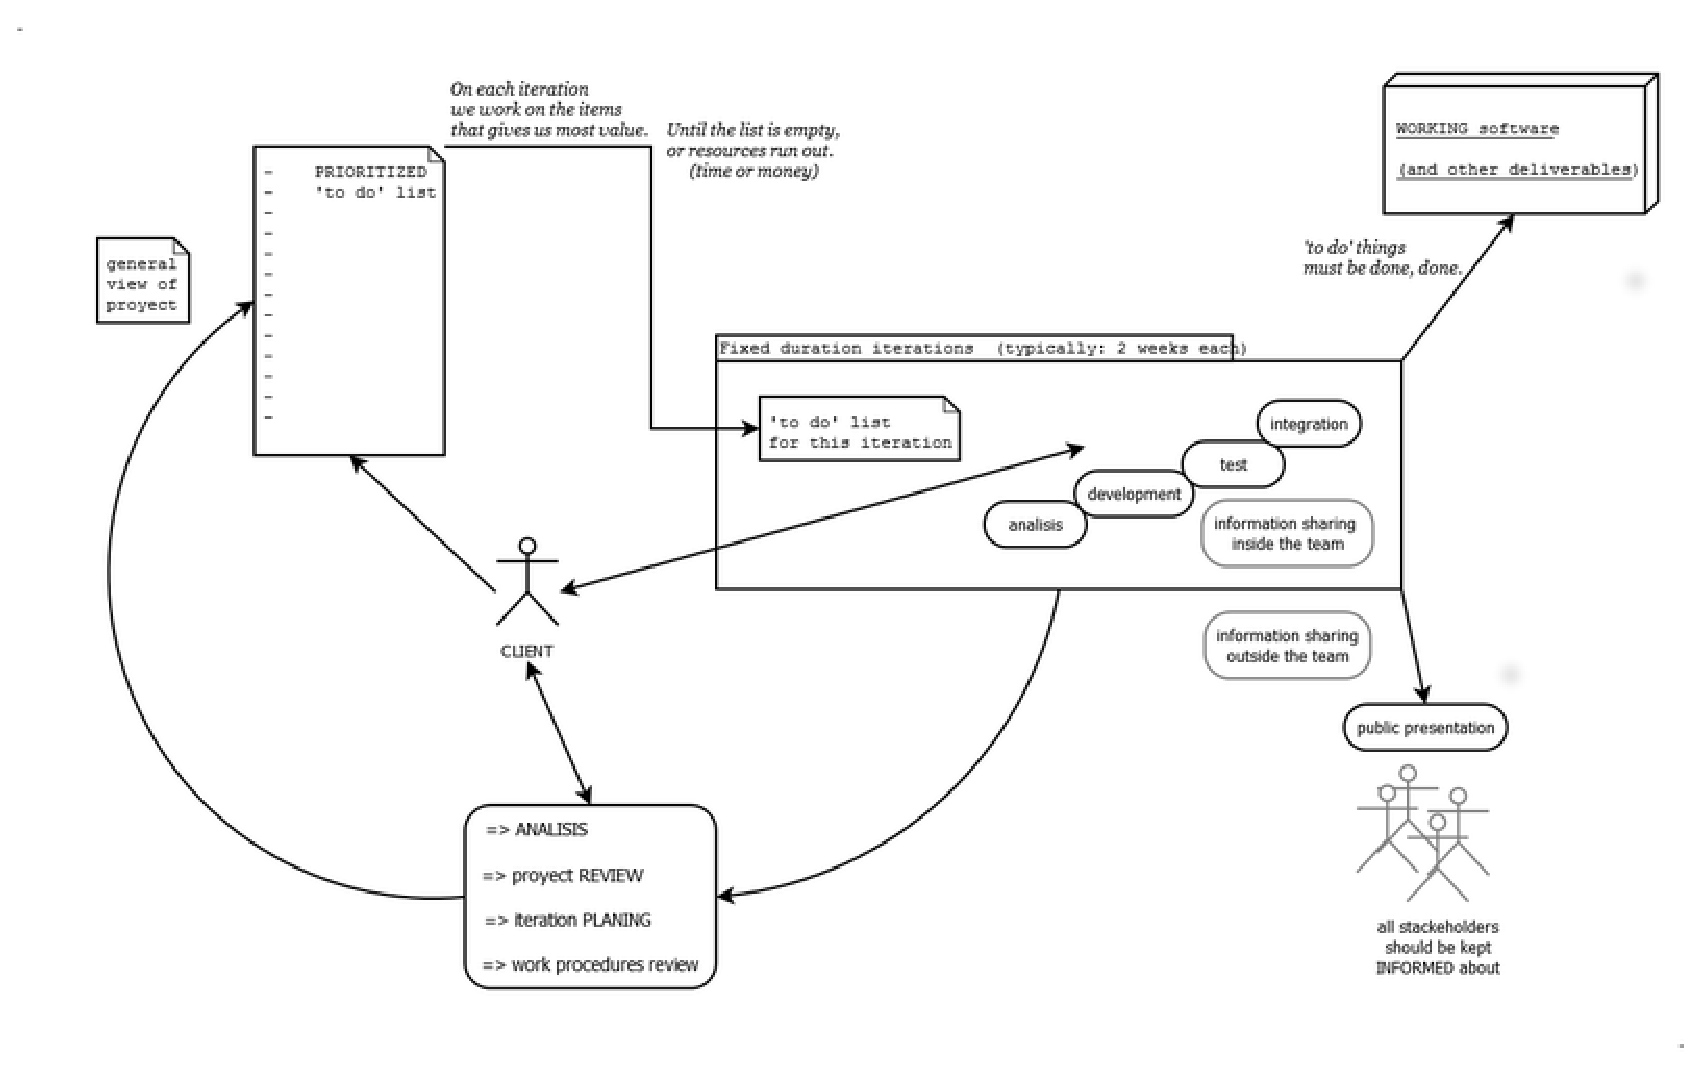
\includegraphics[width=1\columnwidth]{agile_methodology_for_software_development.eps} \label{fig:1-noFCase1}
\end{center}
\caption{Agile Methodology}
\end{figure}

Agile development methods terdefinisi dalam empat nilai, biasa di sebut \textbf{\textit{Agile Alliance’s Manifesto}}. Berikut ini isi dari \textbf{\textit{Agile Alliance’s Manifesto \cite{Agile:01}}} : 

\begin{center}
{\Large \textbf{\textit{Manifesto for Agile Software Development}}}
\end{center}

\textbf{We are uncovering better ways of developing
software by doing it and helping others do it.
Through this work we have come to value:}
\\

\textbf{\Large{Individuals and interactions}}over processes and tools

\textbf{\Large{Working software}} over comprehensive documentation

\textbf{\Large{Customer collaboration}} over contract negotiation

\textbf{\Large{Responding to change over}} following a plan
\\

\textbf{That is, while there is value in the items on
the right, we value the items on the left more.}
\\

Dari \textbf{\textit{Agile Manifesto}} terdefinisi dalam empat nilai :
\begin{itemize}
\item \textbf{Interaksi dan personel} lebih penting daripada proses dan alat.
\item \textbf{Perangkat lunak yang berfungsi} lebih penting daripada dokumentasi yang lengkap.
\item \textbf{Kolaborasi dengan klien} lebih penting daripada negosiasi kontrak.
\item \textbf{Respon terhadap perubahan} lebih penting daripada mengikuti rencana.
\end{itemize}




\subsection{DevOps}
DevOps adalah metode pengembangan software yang menekankan komunikasi, kolaborasi dan integrasi antara pengembang software dan profesional TI dengan menjadikan proses pembuatan software dan perubahan \textit{infrastructure} secara otomatis. Metode ini pertama kali diperkenalkan pada tahun 2008 oleh \textbf{Patrick Debois} pada diskusi nya tentang \textit{"Agile Infrastructure"}, tetapi metode ini baru dikenal sebagai \textit{DevOps} sejavak \textit{DevOpsDay} tahun 2009 di belgia.Bisa disimpulkan DevOps adalah suatu proses \textit{Agile} yang di dukung oleh berbagai \textit{tool} atau infrastructure. 

Dengan \textit{DevOps}, bagian pengembangan dan operasional akan bekerja lebih dekat. Tujuan nya adalah mengurangi friksi antara kedua tim serta meningkatkan kecepatan kerja dengan meng-otomatiskan beberapa proses, sehingga dapat mencapai kinerja optimal. Salah satu lembaga analis ternama di dunia - \textit{Gartner} - merumuskan \textit{DevOps} ini dalam suatu \textit{Blue Print DevOps Architecture}\cite{DevOps:02}.
\\ \\ 

\begin{figure}[htbp]
	\begin{center}
		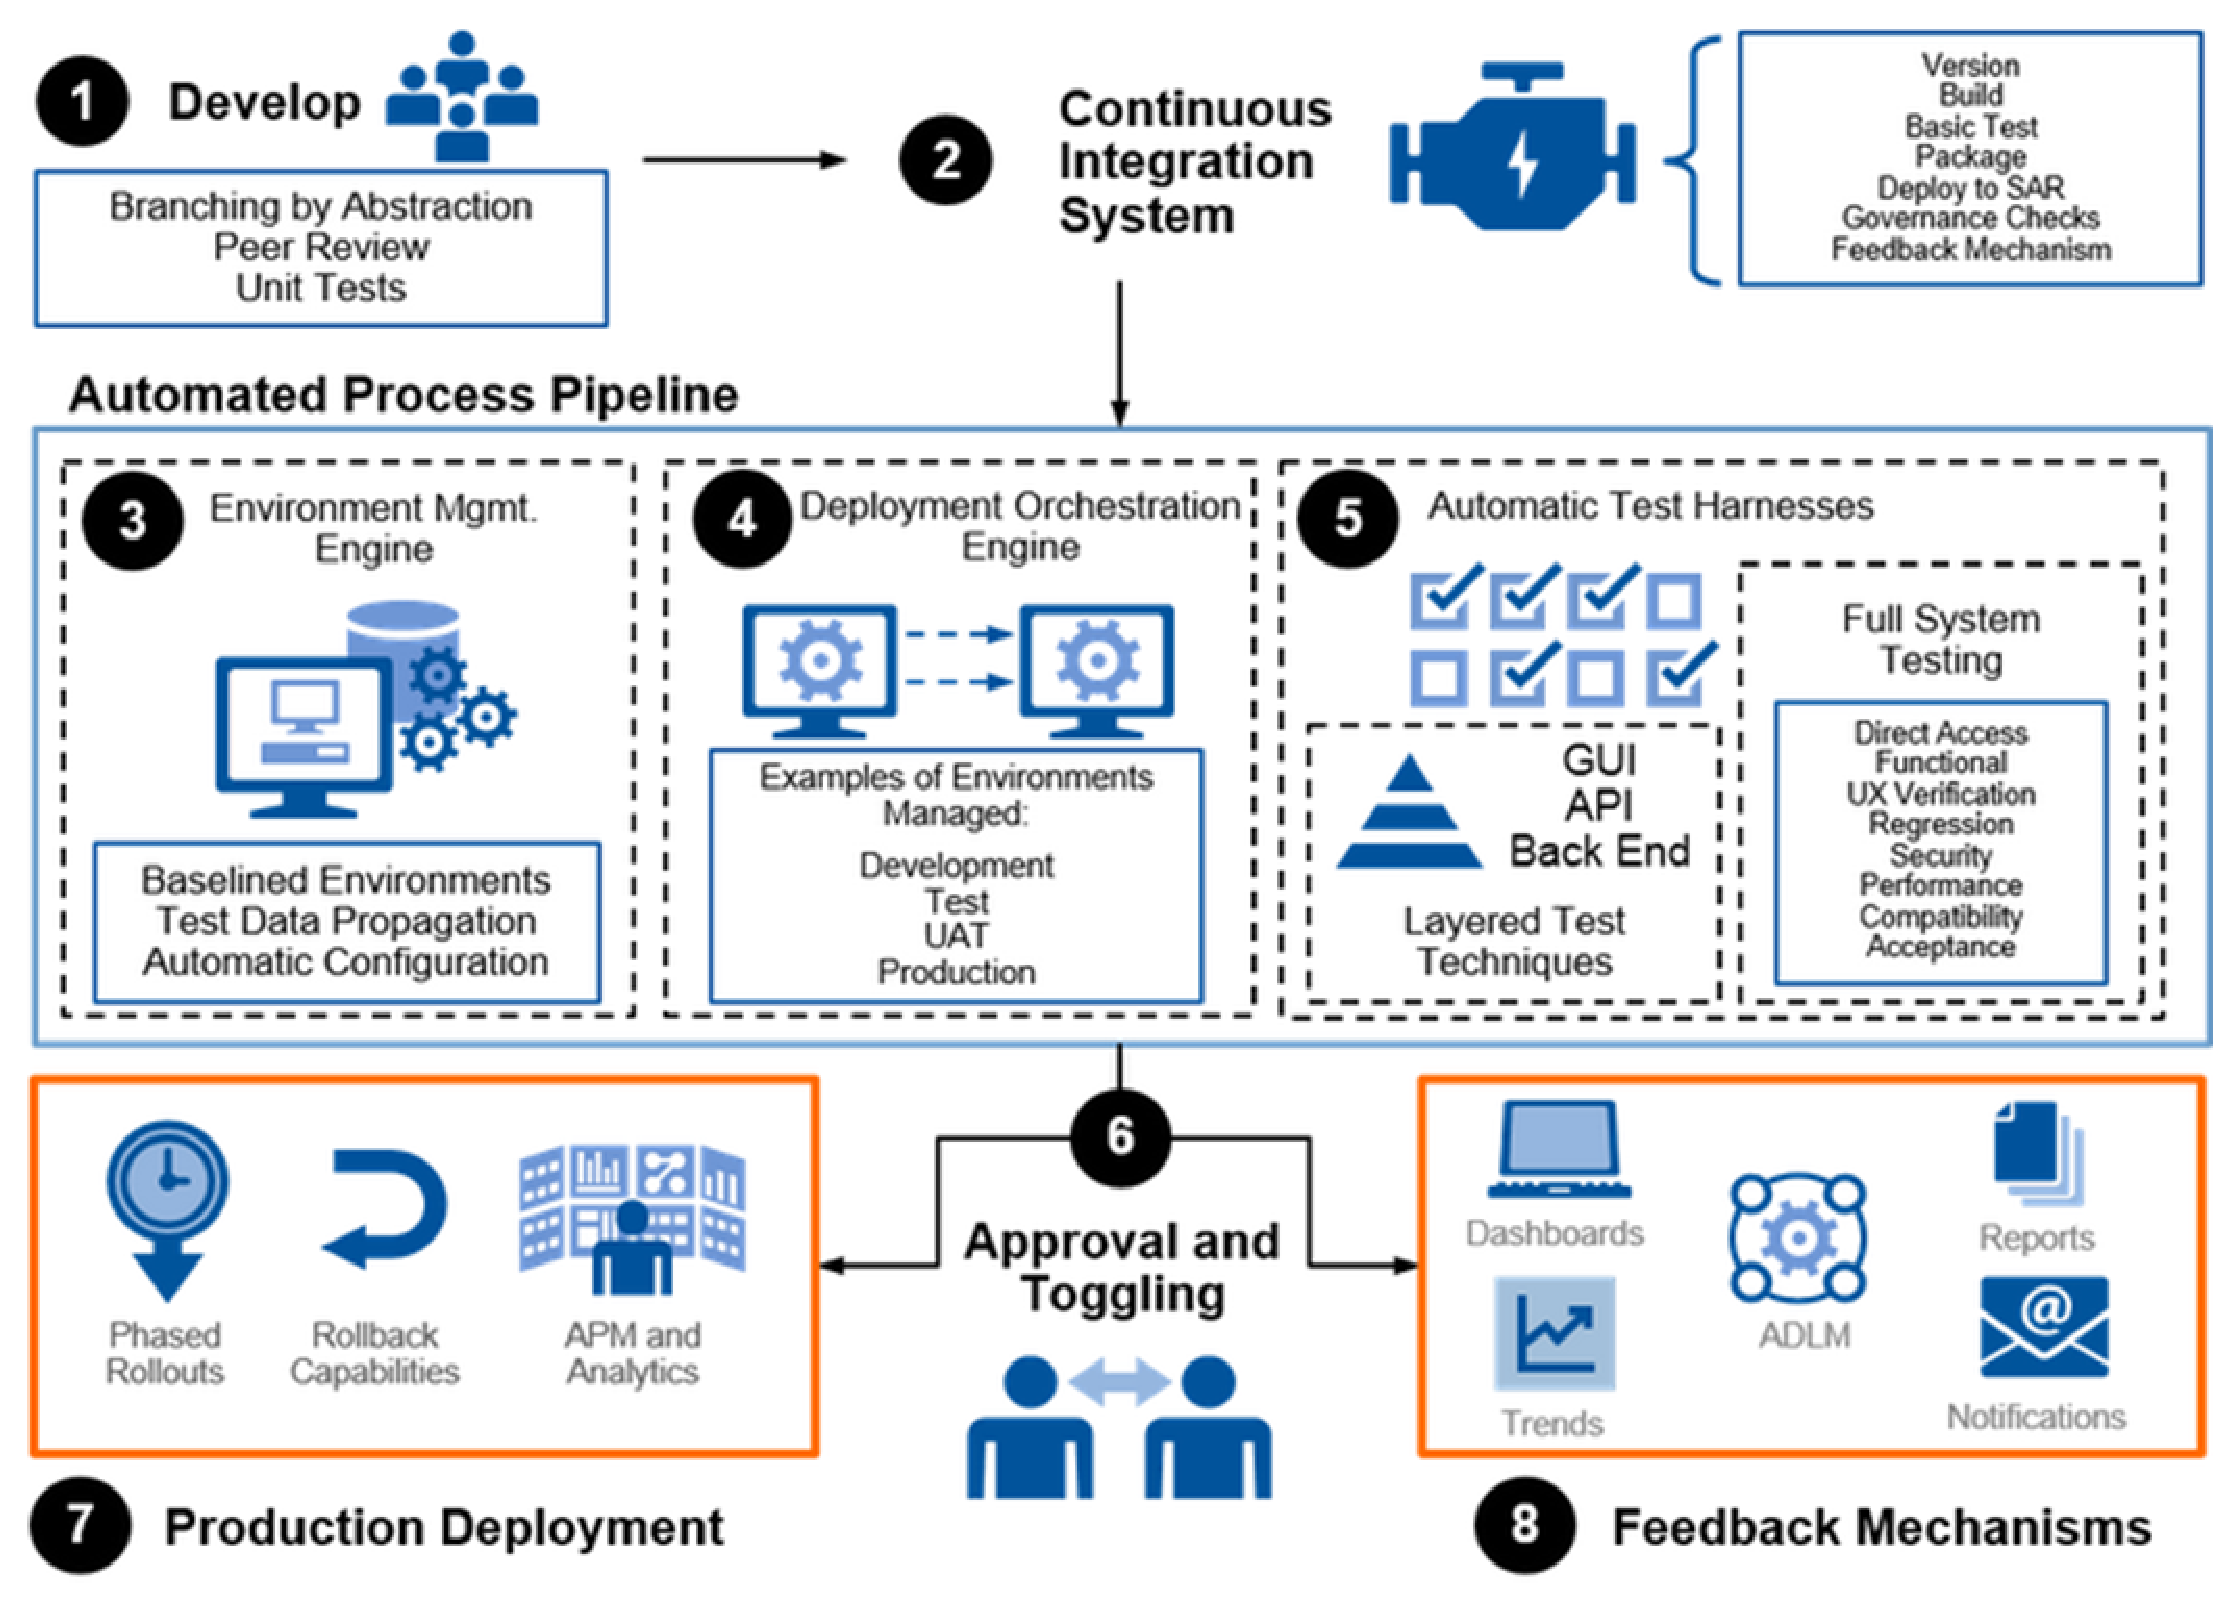
\includegraphics[width=1\columnwidth]{DevOps.eps} \label{fig:1-noFCase1}
	\end{center}
	\caption{DevOps Blueprint Architecture By Gartner}
\end{figure}
    
Di dalam blueprint menggambarkan suatu siklus \textit{software development} yang terdiri atas :
\begin{itemize}
	\item \textit{Software Development Process} dan \textit{versioning system}
	\item \textit{Continuous Integration System}
	\item \textit{Automatic Environment Management Engine}
	\item \textit{Automatic Deployment Orchestration Engine}
	\item \textit{Automatic Test}
	\item \textit{Approval}
	\item \textit{Production Deployment}
	\item \textit{Feedback Mechanism}
\end{itemize}

khusus untuk di pembahasan ini, yang menjadi fokus utama area yang dibahas adalah \textit{Automatic Test}. Berdasarkan \textit{Gartner}, \textit{Automatic test} area di definisikan sebagai :
\textit{Integrate the orchestration engine with automated test frameworks that check quality and efficacy for all aspects of the software-testing process.} \cite{DevOps:02} 
Yang pada prinsip nya adalah \textit{Automatic Test } adalah proses integrasi terhadap suatu test framework dan digunakan untuk cek kualitas dan efisiensi semua aspek yang ada di dalam \textit{software-testing} proses. 
\\ \\ \\ \\ \\ \\ \\ \\ \\ \\ \\ \\ \\ \\ \\ \\ 

\section{Pembahasan}

\subsection{Selenium Web Browser}
Selenium adalah salah satu aplikasi yang digunakan untuk membuat \textit{automated testing} khusus nya untuk aplikasi web. Tool ini pada prinsip nya digunakan oleh seorang \textit{Quality Assurance Engineer} untuk membuat proses testing suatu aplikasi yang berbasi web dibuat secara otomatis. Di tool ini, bisa disiapkan suatu script yang nanti nya akan menjalankan \textit{engine} selenium untuk melakukan tes terhadap aplikasi web secara otomatis bertahap. 

\begin{figure}[htbp]
	\begin{center}
		\includegraphics[width=1\columnwidth]{selenium.eps} \label{fig:1-noFCase1}
	\end{center}
	\caption{Selenium IDE}
\end{figure}


Proses \textit{automated test} ini merupakan salah satu dari komponent yang ada di dalam \textit{DevOps blue print}.  Dengan ada nya komponen ini, target dari \textit{DevOps} yaitu agar mempercepat waktu siklus \textit{development software}  diharapkan bisa tercapai. 

\subsection{Menggunakan Selenium}
Mekanisme \textit{Automated Test} disebut juga \textit{Agile Test}, yaitu software tester berperilaku sebagai end-user dan memeriksa apakah sistemnya dapat berfungsi dengan baik sesuai requirement dari user. 
terjadi nya \textit{Agile Test} tersebut, karena semua aktivitas test direkam oleh sebuah tools, dimana saat melakukan test ulang, bisa secara langsung menjalankan rekaman aktivitas kita, dan tools tersebut akan mengetes ulang secara otomatis. Dalam selenium setiap aktivitas akan terekam masuk ke dalam tiga \textit{tag}, yaitu \textit{command, target, value}. 

\begin{itemize}
	\item \textit{Command}, berisi apa yang dilakukan user pada aplikasi.
	\item \textit{Target}, berisi tujuan dari \textit{command} dilakukan.
	\item \textit{Value}, berisi nilai yang dimasukkan dan di akses saat melakukan test. 
\end{itemize}

\subsubsection{Fitur yang terdapat pada Selenium IDE}
\begin{itemize}
	\item Dapat merekam dan \textit{re-play} hasil rekaman dengan mudah
	\item \textit{Autocomplete} untuk selenium \textit{command}
	\item dapat dijalankan selama testing berlangsung
	\item \textit{Debug} dan \textit{set breakpoint}
	\item bisa disimpan dalam file format berbagai bahasa pemrograman.
	\item mendukung \textit{javascript}
	\item secara otomatis menambahkan \textit{title} pada setiap halaman
\end{itemize}

\subsubsection{Cara Menggunakan Selenium}
Selenium IDE bisa langsung di download sebagai \textit{add-ons} \textbf{mozilla firefox} atau browser lain nya yang mendukung. Selenium IDE ter-integrasi dengan \textit{browser} dan bisa langsung digunakan dengan menuliskan alamat \textit{URL} yang akan ditest, kemudian klik tombol \textit{record}. 

\begin{figure}[htbp]
	\begin{center}
		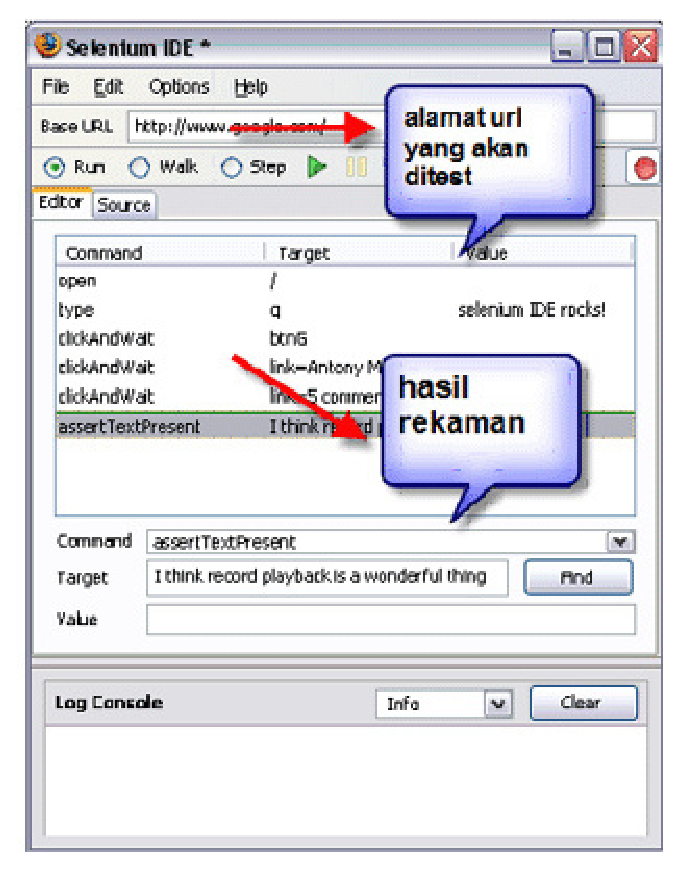
\includegraphics[width=1\columnwidth]{IDE.eps} \label{fig:1-noFCase1}
	\end{center}
	\caption{IDE}
\end{figure}


untuk menjalankan dan mengetes kembali secara otomatis hanya meng-klik tombol \textit{play}.
\\ \\ \\ \\ \\ \\ \\ \\ \\ \\ \\ \\ \\ \\ \\ \\ \\ \\

\begin{figure}[htbp]
	\begin{center}
		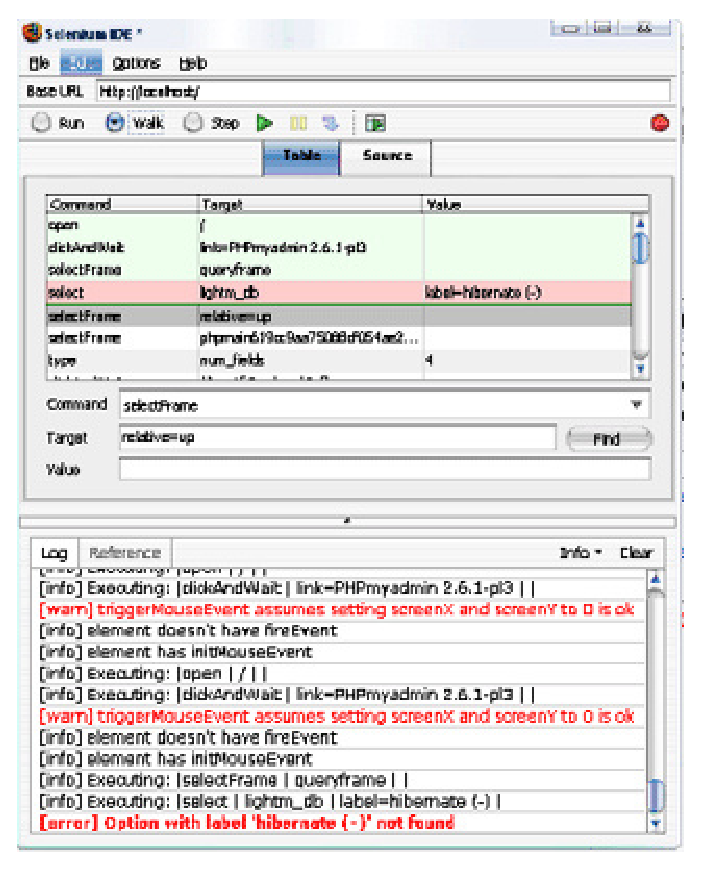
\includegraphics[width=1\columnwidth]{IDE-2.eps} \label{fig:1-noFCase1}
	\end{center}
	\caption{Reply IDE}
\end{figure}



apabila sukses, test akan berwarna hijau, sedangkan kalau gagal, test akan berwarna merah. Kemudian tester menjalankan sistem selayaknya \textit{end-user}, setelah selesai hasilnya bisa disimpan dalam bentuk HTML dan beberapa format yang bisa dipilih seperti pada ilustrasi berikut :
\\ \\ \\ \\ \\ \\ \\ \\ \\ \\ \\ \\ \\ \\ \\ \\ \\ \\
\\ \\ \\ \\ \\ \\ \\ \\ \\ \\ \\ \\ 

\begin{figure}[htbp]
	\begin{center}
		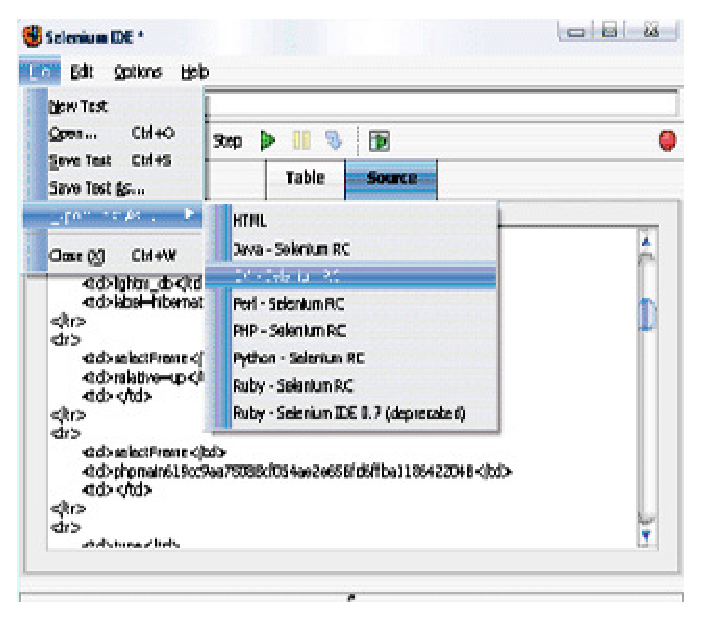
\includegraphics[width=1\columnwidth]{save.eps} \label{fig:1-noFCase1}
	\end{center}
	\caption{save}
\end{figure}

Hasil output \textit{selenium IDE} tadi merupakan satu buah unit test. Kemudian beberapa unit test disatukan dalam suatu \textit{test suite}. \textit{Test Suite} akan  meng-otomatisasi software testing secara keseluruhan. Tools yang digunakan yaitu selenium core. 

 
\section{Kesimpulan}
\subsection{Rangkuman}
\textit{DevOps} sebagai implementasi \textit{Agile Infrastructure} di siklus nya membuat beberapa aktivitas menjadi otomatis. Salah satu nya adalah otomatis testing unit. Untuk mencapai proses otomatis tersebut, maka salah satu tool yang bisa digunakan adalah \textit{Selenium}. Dengan menggunakan \textit{selenium} maka proses testing, terutama untuk aplikasi web, yang sebelum nya hanya dilakukan manual, bisa dilakukan otomatis. Cara nya adalah dengan me-\textit{record} aktivitas testing sebelum nya untuk digunakan di kemudian hari. Sehingga proses nya lebih optimal, dan bisa lebih meng-optimalkan siklus \textit{development}.    
 

\subsection{Saran}
Adapun dari penulisan berikut ini, ada beberapa saran yang penulis rangkum di dalam penulisan ini :
\begin{itemize}
\item Penulis baru menggambarkan relasi antara maturity model, Agile, DevOps dan \textit{Testing Automation}. 
\item Penulis baru menerangkan proses DevOps di siklus \textit{Testing Automation} dengan menggunakan selenium. 
\item Penulis belum menggambarkan perbandingan antara sebelum dan sesudah menggunakan \textit{Automation Testing}. 
\end{itemize}

\section{Daftar Pustaka}


%\bigskip \noindent See \href{link}{Supplement 1} for supporting content.

%\noindent Add citations manually or use BibTeX. See \cite{Zhang:14}.
%\noindent Add citations manually or use BibTeX. See \cite{Agile:01}.
% Bibliography

\bibliography{sample}

%Manual citation list
%\begin{thebibliography}{1}
%\bibitem{Zhang:14}
%Y.~Zhang, S.~Qiao, L.~Sun, Q.~W. Shi, W.~Huang, %L.~Li, and Z.~Yang,
% \enquote{Photoinduced active terahertz metamaterials with nanostructured
%vanadium dioxide film deposited by sol-gel method,} Opt. Express \textbf{22},
%11070--11078 (2014).
%\end{thebibliography}

\end{document}